\documentclass[11pt,letter]{article}
%-------------------------
\usepackage{amsmath,amssymb}

\usepackage{amsthm}
\usepackage{mathrsfs}
\usepackage{bm}
\usepackage{ascmac} 
\usepackage{amsmath}
\usepackage{natbib} %
\usepackage{fancybox}
\usepackage{float}
\usepackage{booktabs} 
\usepackage{bm,xstring}
\usepackage{tabularx}
\usepackage{graphicx}
%\usepackage{mediabb}
\usepackage{lipsum}
\usepackage {pdfpages}
\usepackage{booktabs}
\usepackage{array}
\usepackage{paralist}
\usepackage{verbatim}
\usepackage{subfig} 
\usepackage{ascmac}
\usepackage{amsthm}
\usepackage{multirow}
\usepackage{amsmath}
\usepackage{natbib}
\usepackage{longtable}
\usepackage{hhline}
\usepackage{tabularx}
\usepackage{booktabs}
%\usepackage[T1]{fontenc}
\usepackage{textcomp}
\usepackage{here}
\usepackage{setspace}
\usepackage{color}
\usepackage{url}
\usepackage{xcolor}
%\usepackage{filecontents}
\usepackage{setspace}
\usepackage{fancyhdr}
\usepackage{titling}
\usepackage{titlesec}
\usepackage{sectsty}
\usepackage{listings}
\usepackage[many]{tcolorbox}
\usepackage[framemethod=TikZ]{mdframed}
\usepackage[dvipdfmx]{}
%\usepackage[dvipdfmx]{color}
\usepackage{epstopdf}
%\usepackage[dvipdfmx]{color}

\usepackage{bbm}
\usepackage{pdflscape}
\newcommand{\vect}[1]{\boldsymbol{\mathbf{#1}}}

%%%%%%%%%%%%%%%%%%%%%%%%%%%%%%
%Theorem
\newcounter{theo}[section] \setcounter{theo}{0}
\renewcommand{\thetheo}{\arabic{theo}}
\newenvironment{theo}[2][]{%
\refstepcounter{theo}%
\ifstrempty{#1}%
{\mdfsetup{%
frametitle={%
\tikz[baseline=(current bounding box.east),outer sep=0pt]
\node[anchor=east,rectangle,fill=gray!20]
{\strut Theorem~\thetheo};}}
}%
{\mdfsetup{%
frametitle={%
\tikz[baseline=(current bounding box.east),outer sep=0pt]
\node[anchor=east,rectangle,fill=gray!20]
{\strut Theorem~\thetheo:~#1};}}%
}%
\mdfsetup{innertopmargin=10pt,linecolor=gray!20,%
linewidth=2pt,topline=true,%
frametitleaboveskip=\dimexpr-\ht\strutbox\relax
}
\begin{mdframed}[]\relax%
\label{#2}}{\end{mdframed}}
%%%%%%%%%%%%%%%%%%%%%%%%%%%%%%
%Lemma
\newcounter{lem}[section] \setcounter{lem}{0}
\renewcommand{\thelem}{\arabic{section}.\arabic{lem}}
\newenvironment{lem}[2][]{%
\refstepcounter{lem}%
\ifstrempty{#1}%
{\mdfsetup{%
frametitle={%
\tikz[baseline=(current bounding box.east),outer sep=0pt]
\node[anchor=east,rectangle,fill=gray!50]
{\strut Lemma~\thelem};}}
}%
{\mdfsetup{%
frametitle={%
\tikz[baseline=(current bounding box.east),outer sep=0pt]
\node[anchor=east,rectangle,fill=gray!50]
{\strut Lemma~\thelem:~#1};}}%
}%
\mdfsetup{innertopmargin=10pt,linecolor=gray!50,%
linewidth=2pt,topline=true,%
frametitleaboveskip=\dimexpr-\ht\strutbox\relax
}
\begin{mdframed}[]\relax%
\label{#2}}{\end{mdframed}}
%%%%%%%%%%%%%%%%%%%%%%%%%%%%%%
%Assumption
\newcounter{asm}[section] \setcounter{asm}{0}
\renewcommand{\theasm}{\arabic{section}.\arabic{asm}}
\newenvironment{asm}[2][]{%
\refstepcounter{asm}%
\ifstrempty{#1}%
{\mdfsetup{%
frametitle={%
\tikz[baseline=(current bounding box.east),outer sep=0pt]
\node[anchor=east,rectangle,fill=gray!50]
{\strut Assumption~\theasm};}}
}%
{\mdfsetup{%
frametitle={%
\tikz[baseline=(current bounding box.east),outer sep=0pt]
\node[anchor=east,rectangle,fill=gray!50]
{\strut Assumption~\thelem:~#1};}}%
}%
\mdfsetup{innertopmargin=10pt,linecolor=gray!50,%
linewidth=2pt,topline=true,%
frametitleaboveskip=\dimexpr-\ht\strutbox\relax
}
\begin{mdframed}[]\relax%
\label{#2}}{\end{mdframed}}
%%%%%%%%%%%%%%%%%%%%%%%%%%%%%%
%Definition
\newcounter{defn}[section] \setcounter{defn}{0}
\renewcommand{\thedefn}{\arabic{section}.\arabic{defn}}
%\renewcommand{\thedefn}{\arabic{defn}}
\newenvironment{defn}[2][]{%
\refstepcounter{defn}%
\ifstrempty{#1}%
{\mdfsetup{%
frametitle={%
\tikz[baseline=(current bounding box.east),outer sep=0pt]
\node[anchor=east,rectangle,fill=gray!50]
{\strut Definition~\thedefn};}}
}%
{\mdfsetup{%
frametitle={%
\tikz[baseline=(current bounding box.east),outer sep=0pt]
\node[anchor=east,rectangle,fill=gray!50]
{\strut Definition~\thedefn:~#1};}}%
}%
\mdfsetup{innertopmargin=10pt,linecolor=gray!50,%
linewidth=2pt,topline=true,%
frametitleaboveskip=\dimexpr-\ht\strutbox\relax
}
\begin{mdframed}[]\relax%
\label{#2}}{\end{mdframed}}

%%%%%%%%%%%%%%%%%%%%%%%%%%%%%%
%Proof
\newcounter{prf}[section]\setcounter{prf}{0}
\renewcommand{\theprf}{\arabic{section}.\arabic{prf}}
\newenvironment{prf}[2][]{%
\refstepcounter{prf}%
\ifstrempty{#1}%
{\mdfsetup{%
frametitle={%
\tikz[baseline=(current bounding box.east),outer sep=0pt]
\node[anchor=east,rectangle,fill=gray!50]
{\strut Proof~\theprf};}}
}%
{\mdfsetup{%
frametitle={%
\tikz[baseline=(current bounding box.east),outer sep=0pt]
\node[anchor=east,rectangle,fill=gray!50]
{\strut Proof~\theprf:~#1};}}%
}%
\mdfsetup{innertopmargin=10pt,linecolor=gray!50,%
linewidth=2pt,topline=true,%
frametitleaboveskip=\dimexpr-\ht\strutbox\relax
}
\begin{mdframed}[]\relax%
\label{#2}}{\qed\end{mdframed}}
%%%%%%%%%%%%%%%%%%%%%%%%%%%%%%
%%%%%%%%%%%%%%%%%%%%%%%%%%%%%%
%Note
\newcounter{notes}[section] \setcounter{notes}{0}
\renewcommand{\thenotes}{\arabic{notes}}
\newenvironment{notes}[2][]{%
\refstepcounter{notes}%
\ifstrempty{#1}%
{\mdfsetup{%
frametitle={%
\tikz[baseline=(current bounding box.east),outer sep=0pt]
\node[anchor=east,rectangle,fill=gray!50]
{\strut Note~\thenotes};}}
}%
{\mdfsetup{%
frametitle={%
\tikz[baseline=(current bounding box.east),outer sep=0pt]
\node[anchor=east,rectangle,fill=gray!50]
{\strut Note~\thenotes:~#1};}}%
}%
\mdfsetup{innertopmargin=10pt,linecolor=gray!50,%
linewidth=2pt,topline=true,%
frametitleaboveskip=\dimexpr-\ht\strutbox\relax
}
\begin{mdframed}[]\relax%
\label{#2}}{\end{mdframed}}

\newtcolorbox{myboxi}[1][]{
  breakable,
  title=#1,
  colback=white,
  colbacktitle=white,
  coltitle=black,
  fonttitle=\bfseries,
  bottomrule=0pt,
  toprule=0pt,
  leftrule=3pt,
  rightrule=3pt,
  titlerule=0pt,
  arc=0pt,
  outer arc=0pt,
  colframe=black,
}


\usepackage{tgpagella}

\definecolor{mygreen}{RGB}{28,172,0} % color values Red, Green, Blue
\definecolor{mylilas}{RGB}{170,55,241}
\lstset{language=Matlab,%
    %basicstyle=\color{red},
    breaklines=true,%
    morekeywords={matlab2tikz},
    keywordstyle=\color{blue},%
    morekeywords=[2]{1}, keywordstyle=[2]{\color{black}},
    identifierstyle=\color{black},%
    stringstyle=\color{mylilas},
    commentstyle=\color{mygreen},%
    showstringspaces=false,%without this there will be a symbol in the places where there is a space
    numbers=left,%
    numberstyle={\tiny \color{black}},% size of the numbers
    numbersep=9pt, % this defines how far the numbers are from the text
    emph=[1]{for,end,break},emphstyle=[1]\color{red}, %some words to emphasise
    %emph=[2]{word1,word2}, emphstyle=[2]{style},    
}

%\usepackage[none]{hyphenat}
\usepackage{geometry}
\geometry{left=1in,right=1in, top=1in,bottom=1in}
\setlength\parindent{0pt}
%\renewcommand{\thesubsection}{(\alph{subsection})}
\usepackage{fancyhdr}
 

%\usepackage[shortlabels]{enumitem}
%                    \setlist[enumerate, 1]{1\textsuperscript{o}}


%--------------Shortcuts-----------
%Expectation
\newcommand{\Exp}[1]{\mathbb{E}\left[{#1}\right]}
\newcommand{\Var}[1]{\text{Var}\left[{#1}\right]}
\newcommand{\AsymVar}[1]{\text{AsymVar}\left[{#1}\right]}
\newcommand{\cov}[1]{\text{cov}\left[{#1}\right]}
\newcommand{\plim}[1]{\text{plim}\{{#1}\}}
\newcommand{\Ind}[1]{\mathbbm{1}\{{#1}\}}
\newcommand{\Prob}[1]{\text{Pr}\left({#1}\right)}
%hat
\newcommand{\h}[1]{\hat{#1}}
\newcommand{\thetahat}{\hat{\theta}}
\newcommand{\thetabar}{\overline{\theta}}
\newcommand{\gbar}{\overline{g}}
\newcommand{\psihat}{\hat{\psi}}

\newcommand{\vecty}{\vect{y}}

%upper and lower ber
\newcommand{\ob}[1]{\overline{#1}}
\newcommand{\ub}[1]{\underline{#1}}
\newcommand{\taubar}{\overline{\tau}}

%epsilon
\newcommand{\epsi}{\varepsilon}
\def\checkmark{\tikz\fill[scale=0.4](0,.35) -- (.25,0) -- (1,.7) -- (.25,.15) -- cycle;} 

\newcommand{\nonum}{\nonumber}

%ln()
\newcommand{\lnp}[1]{\ln\left({#1}\right)}

% parenthesis
\newcommand{\prn}[1]{\left({#1}\right)}
\newcommand{\mprn}[1]{\{{#1}\}}
\newcommand{\lmprn}[1]{\big\{{#1}\big\}}
\newcommand{\Lmprn}[1]{\Big\{{#1}\Big\}}
\newcommand{\llmprn}[1]{\biggl\{{#1}\biggr\}}
\newcommand{\LLmprn}[1]{\Biggl\{{#1}\Biggr\}}
\newcommand{\lprn}[1]{\left[{#1}\right]}

% cfrac
\newcommand{\cf}[2]{\cfrac{#1}{#2}}

% convergence in probability
\newcommand{\conp}{\xrightarrow{p}}
\newcommand{\cond}{\xrightarrow{d}}
\newcommand{\as}{\xrightarrow{a.s.}}

% Norm
\newcommand{\norm}[1]{\left\lVert{#1}\right\rVert}
\newcommand{\abs}[1]{\left\lvert{#1}\right\rvert}

\newcommand{\rootn}{\sqrt{n}}

\newcommand{\note}[1]{\ \ \ \ \text{#1}}

\newcommand{\ave}[1]{\frac{1}{#1}\sum_{i=1}^{#1}}

\newcommand{\half}{\cfrac{1}{2}}
\newcommand{\pihat}{\hat{\pi}}

\newcommand{\mbf}[1]{\mathbf{#1}}

\DeclareMathOperator*{\argmax}{argmax} 
\DeclareMathOperator*{\argmin}{argmin} 
\DeclareMathOperator*{\arginf}{arginf} 

\newcommand{\pmat}[1]{\begin{pmatrix} #1 \end{pmatrix}}%
\newcommand{\bmat}[1]{\begin{bmatrix} #1 \end{bmatrix}}%

\pagestyle{fancy}
\fancyhf{}
\chead{ECON512 Homework 2 -- Kensuke Suzuki}
\lhead{}
\rfoot{\thepage}

\allowdisplaybreaks
\setstretch{1}

\newtheorem{definition}{Definition}

\newtheorem{lemma}{Lemma}
\newtheorem{assumption}{Assumption}
\newtheorem{theorem}{Theorem}

\newcommand{\code}[1]{\texttt{#1}}

\bibliographystyle{aer} 

%----------------------------------------------------------------------------------------
%	TITLE SECTION
%----------------------------------------------------------------------------------------

\newcommand{\horrule}[1]{\rule{\linewidth}{#1}} % Create horizontal rule command with 1 argument of height

\title{	
\normalfont \normalsize 
\textsc{Penn State, Fall 2018, ECON512 Empirical Method} \\ [25pt] % Your university, school and/or department name(s)
\horrule{0.5pt} \\[0.4cm] % Thin top horizontal rule
\huge Homework 3 \\ % The assignment title
\horrule{2pt} \\[0.5cm] % Thick bottom horizontal rule
}

\author{Kensuke Suzuki} % Your name

\date{\normalsize\today} % Today's date or a custom date

\begin{document}

\maketitle % Print the title


%%%%%%%%%%%%%%%%%%%%%%
\section*{Problem 1}

First define the function \code{TobitLLF.m} which gives the (negative of) log likelihood for given vector of $\beta$, $\vect{X}$ and $\vect{y}$.


\lstinputlisting{TobitLLF.m}

Given the vector of $\vect{X}$ and $\vect{y}$, we re-define anonymous function of $\beta$ which we will minimize with respect to the vector of $\beta$.

In the first question, we use the Nelder-Mead method. Following the course material, we use the build-in optimizer \code{fminsearch}. 

For the initial value, we use $\beta_0 = \lprn{\log\frac{\sum_i y_i}{n},0,0,0,0,0}^\top$. Optimization algorithm yields the MLE estimates:

\begin{align*}
\beta = \lprn{
\begin{array}{r}
 2.5339 \\
-0.0323\\
0.1157\\
-0.3540\\
0.0798\\
-0.4094
\end{array}
}
\end{align*}

The figure below shows the function values along the iteration. 

\begin{center}
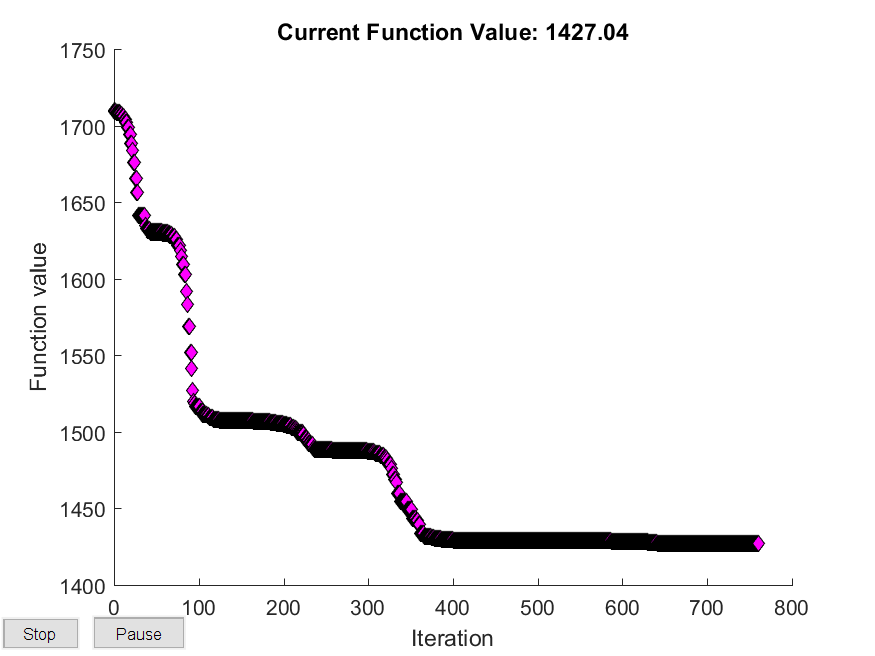
\includegraphics[width=0.7\textwidth]{q1.png} 
\end{center}

%%%%%%%%%%%%%%%%%%%%%%
\section*{Problem 2}

In this question, we use the build-in optimizer \code{fminunc}, where the default algorithm is quasi-Newton method. The algorithm found the local minimum as the size of the gradient is less than the tolerance. Estimated MLE estimates are:


\begin{align*}
\beta = \lprn{
\begin{array}{r}
 2.5339 \\
-0.0323\\
0.1157\\
-0.3540\\
0.0798\\
-0.4094
\end{array}
}
\end{align*}

The estimates are same as in the question 1.

%%%%%%%%%%%%%%%%%%%%%%
\section*{Problem 3}

We now define the function returning the (negative of) sum of squared residuals, \code{NlsRSS}.


\lstinputlisting{NlsRSS.m}

Given vector of $\vec{X}$ and $\vect{y}$, we define the anonymous function of $\beta$ which we minimize. 

We use the same initial value for $\beta$. As we discussed in the last question, the estimates are greatly affected by the initial guess.


For this question, we use the built-in optimizer \code{lsqnonlin}. The results are:

\begin{align*}
\beta = 
 \lprn{
\begin{array}{r}
0.3755 \\
-0.0119 \\
0.0856 \\
-0.0503 \\
0.0187 \\
-0.0745 \\
\end{array}
}
\end{align*}


%%%%%%%%%%%%%%%%%%%%%%
\section*{Problem 4}

In this question, we employ the Nelder-Mead method using \code{fminsearch}. Initial value for $\beta$ is same as before. Again, as we discussed below, the results are greatly affected by the initial values. The optimization yields:

\begin{align*}
\beta = 
 \lprn{
\begin{array}{r}
345.9665 \\
1.2039 \\
-7.8108 \\
1.8421 \\
-0.5917 \\
0.9241
\end{array}
}
\end{align*}



%%%%%%%%%%%%%%%%%%%%%%
\section*{Problem 5}

For each method, we minimizes the function value with different initial values for $\beta$ and see how the results are affected by the initial values. For here, we change the initial values for $\beta_0$ from 1 to 5 (with step 0.2) and keep $\beta_i = 0$ for $i=1,...,5$

\subsection*{MLE with Nelder-Mead (Figure 1)}
Figure 1 shows the estimated coefficients with different initial values for $\beta_0$. It is clear from the figure that the estimates vary substantially with different initial values. The response of estimates seems to be random to the initial values.

\subsection*{MLE with Quasi-Newton (Figure 2)}
Figure 2 is the result with Quasi-Newton method. Unlike the Nelder-Mead method, the Quasi-Newton method yields fairly stable results. It implies that the results are not substantially affected by the initial values. 

\subsection*{NLS with \code{lsqnonlin} (Figure 3)}
Again the results are greatly affected by the initial values but the figure reveals (unlike the case in the Nelder-Mead presented below) linear relationship between the estimates and initial values. 

\subsection*{NLS with Nelder-Mead (Figure 4)}
Finally, the figure 4 demonstrates the results for NLS with Nelder-Mead. The left y-axis is the coefficients for $\beta_0$ and the right y-axis is for the rest of the parameters.  As in Figure 1, it reveals that the initial values matter in the Nelder-Mead method. We find (in particular for $\beta_0$) mostly random fluctuation in the results with different initial values.


\subsection*{Discussion:}

\begin{figure}
\begin{center}
\caption{MLE with Nelder-Mead}
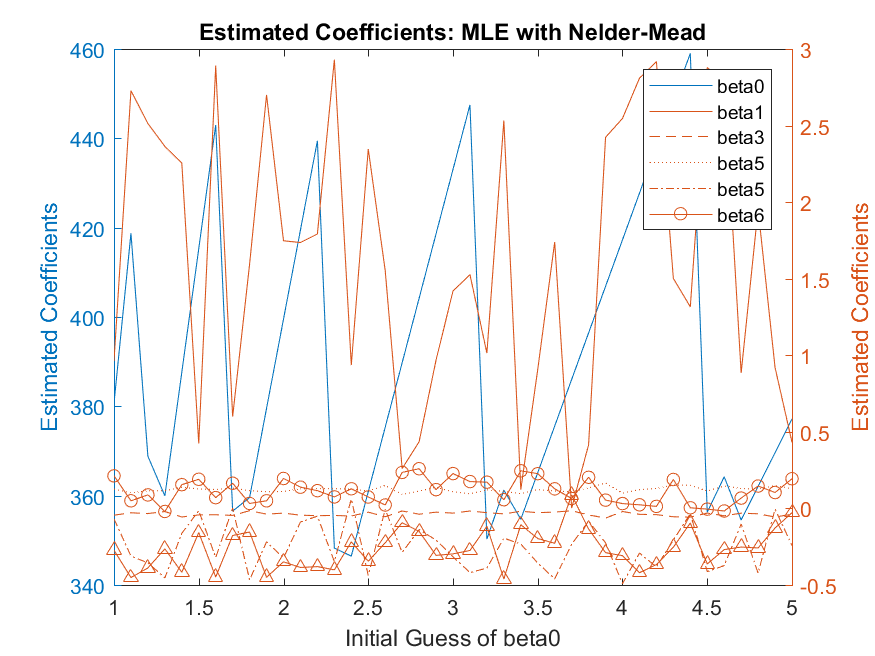
\includegraphics[width=0.7\textwidth]{MLE_NM.png} 
\end{center}
\end{figure}

\begin{figure}
\begin{center}
\caption{MLE with Quasi-Newton}
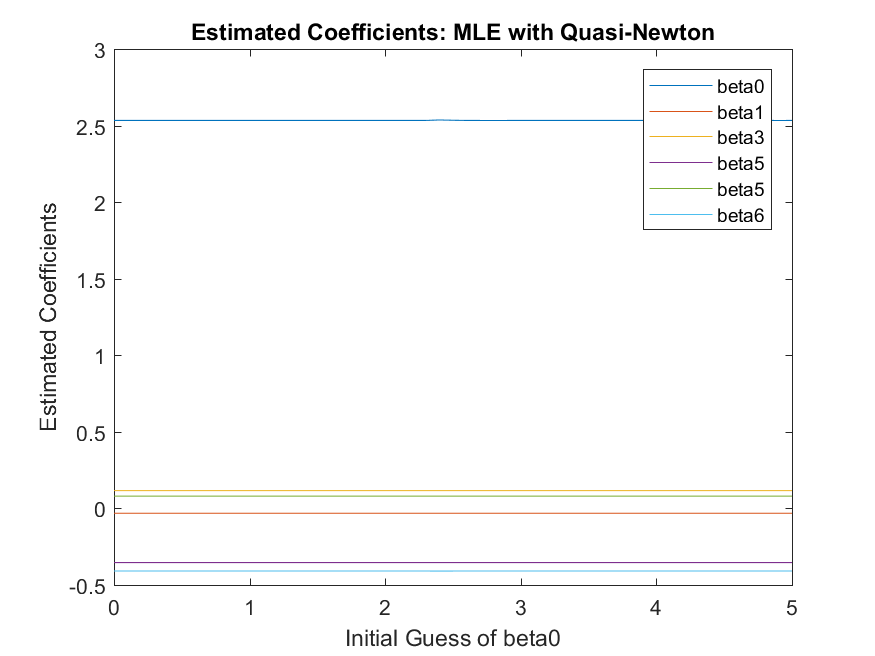
\includegraphics[width=0.7\textwidth]{MLE_QN.png} 
\end{center}
\end{figure}


\begin{figure}
\begin{center}
\caption{NLS with lsqnonlin}
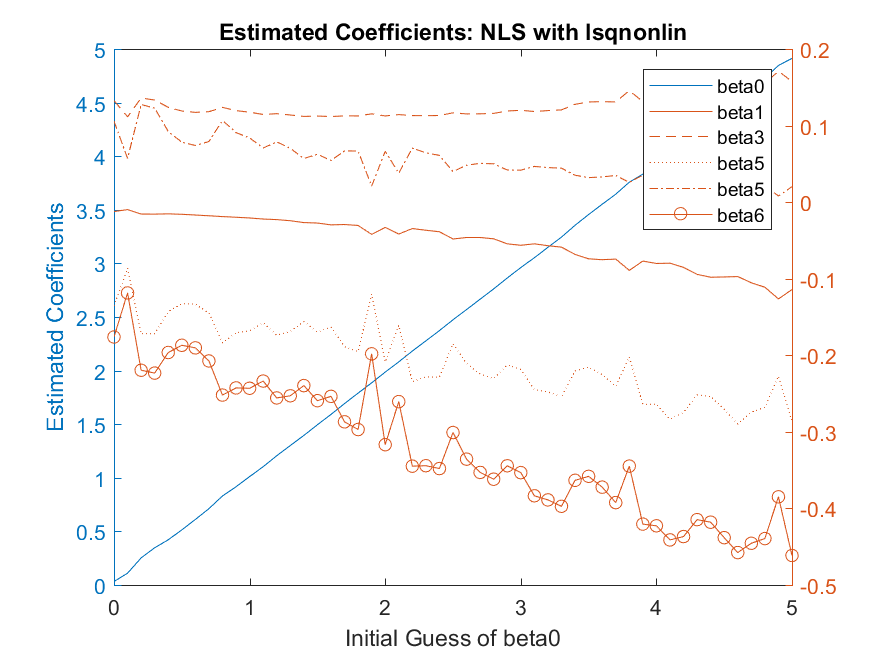
\includegraphics[width=0.7\textwidth]{NLS_lsqnonlin.png} 
\end{center}
\end{figure}

\begin{figure}
\begin{center}
\caption{NLS with Nelder-Mead}
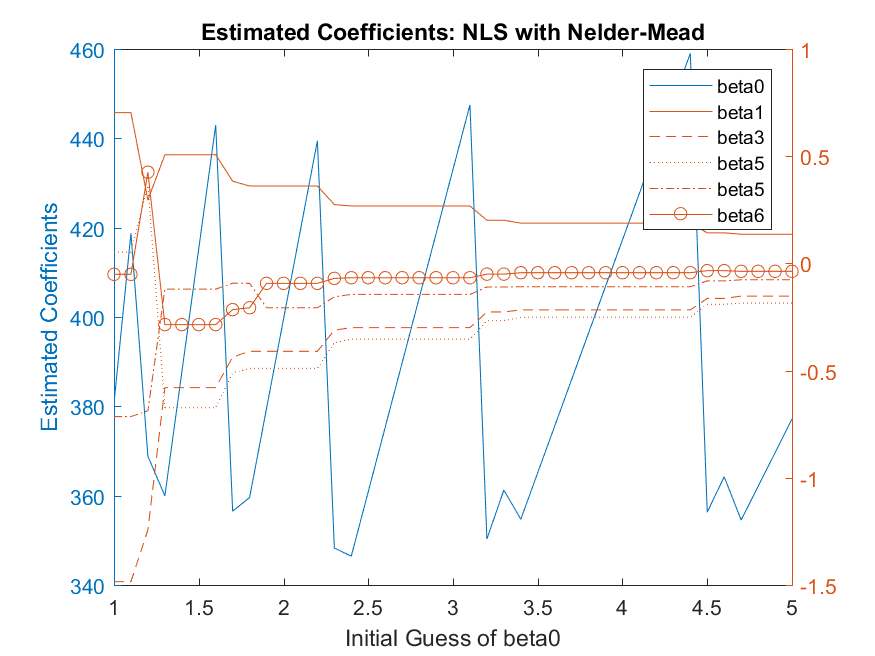
\includegraphics[width=0.7\textwidth]{NLS_NM.png} 
\end{center}
\end{figure}






%%%%%%%%%%%%%%%%%%%%%%
\section*{Matlab Code}
\lstinputlisting{HW3.m}


\end{document}  



  